\subsection{Methane pyrolysis in shock-tube using constant pressure reactor}
The pyrolysis of 5\% $\mathrm{CH_4}$-Ar was investigated using a constant pressure reactor model (CPR) for the post-shock temperature, $\mathrm{T_5}$ range of 1800-3000 K, and pressure, $\mathrm{P_5}$ range of 4.7-7.1 bar. $P_5$ was not specified for each experiment (characterized with $\mathrm{T_5}$), so we assume that $\mathrm{P_5}$ linearly increases with $\mathrm{T_5}$ in the specified pressure range~\citep{agafonov2016unified}. Caltech mechanism was used to describe gas chemistry. The inception and PAH adsorption rates were adjusted using $\eta_{inc}$ and $\eta_{ads}$, respectively to match the predicted carbon yield at t=1.5 ms over the studied $\mathrm{T_5}$ and $\mathrm{P_5}$ with the light extinction measurements at $\mathrm{\lambda}$=632~nm~\citep{agafonov2016unified}. The measured carbon yield (CY) was retrieved from the reported CY$\times$E(m). There are uncertainties in the CY calculated using this technique due to the variability of E(m). It is common to use a E(m) of mature soot which might not be accurate for soot particles formed in shock-tube in short residence times ($\approx$ 2 ms), but the E(m) of soot increases significantly with particle size, composition and maturity. For example, E(m) changes from 0.05 to 0.25 as their primary particle diameter grows to 20 nm within 1.6 ms of acetylene pyrolysis in a shock tube. Having said that, there is still a large gap in the quantitative understanding evolving E(m) of soot. We considered the variability of E(m) from 0.174~\citep{lee1981optical} to 0.37~\citep{agafonov2011soot} in the literature. 

A parametric study was performed on the inception and adsorption adjustment factors using a grid search approach. Each factor was varied across 11 logarithmically spaced values ranging from $10^{-4}$ to 1, resulting in 99 simulation cases for each data point (792 simulations in total). The combinations of $\eta_{inc}$ and $\eta_{ads}$ were sorted using the average relative error for all data points to find the combinations(s) of adjustment factors resulting in the minimum prediction error for carbon yield. Figure~\ref{fig:shockagof_yielderror_cpr} shows a heat map of the mean relative error normalized by the maximum value for Reactive Dimerization. The largest error occurs for the combination of the maximum inception and minimum PAH adsorption corresponding to  $\eta_{inc}=1$ ($\mathrm{\log_{10}}(\eta_{inc})$ = 0) and $\eta_{ads}=10^{-4}$ ($\mathrm{\log_{10}}(\eta_{ads})$ = -4). The region with the lowest normalized error (less than 5\%) was outlined in blue, and it covers a large number of adjustment factor pairs that led to the accurate prediction of carbon yield, but might change the predicted morphology. To better understand these effect, we took a multi-step approach: i) the model was run without soot to focus on the chemistry of precursors and $\mathrm{C_2H_2}$, ii) the inception models were optimized using equal adjustment factors $\eta_{inc}$=$\eta_{ads}$ iii) the inception models were optimized with the minimum adsorption rate, $\eta_{ads}= 10^{-4}$ (labeled as \textit{Min Ads}) and the minimum inception flux, $\eta_{inc}= 10^{-4}$ (labeled as \textit{Min Ads}).

\begin{figure}[H]
	\centering
	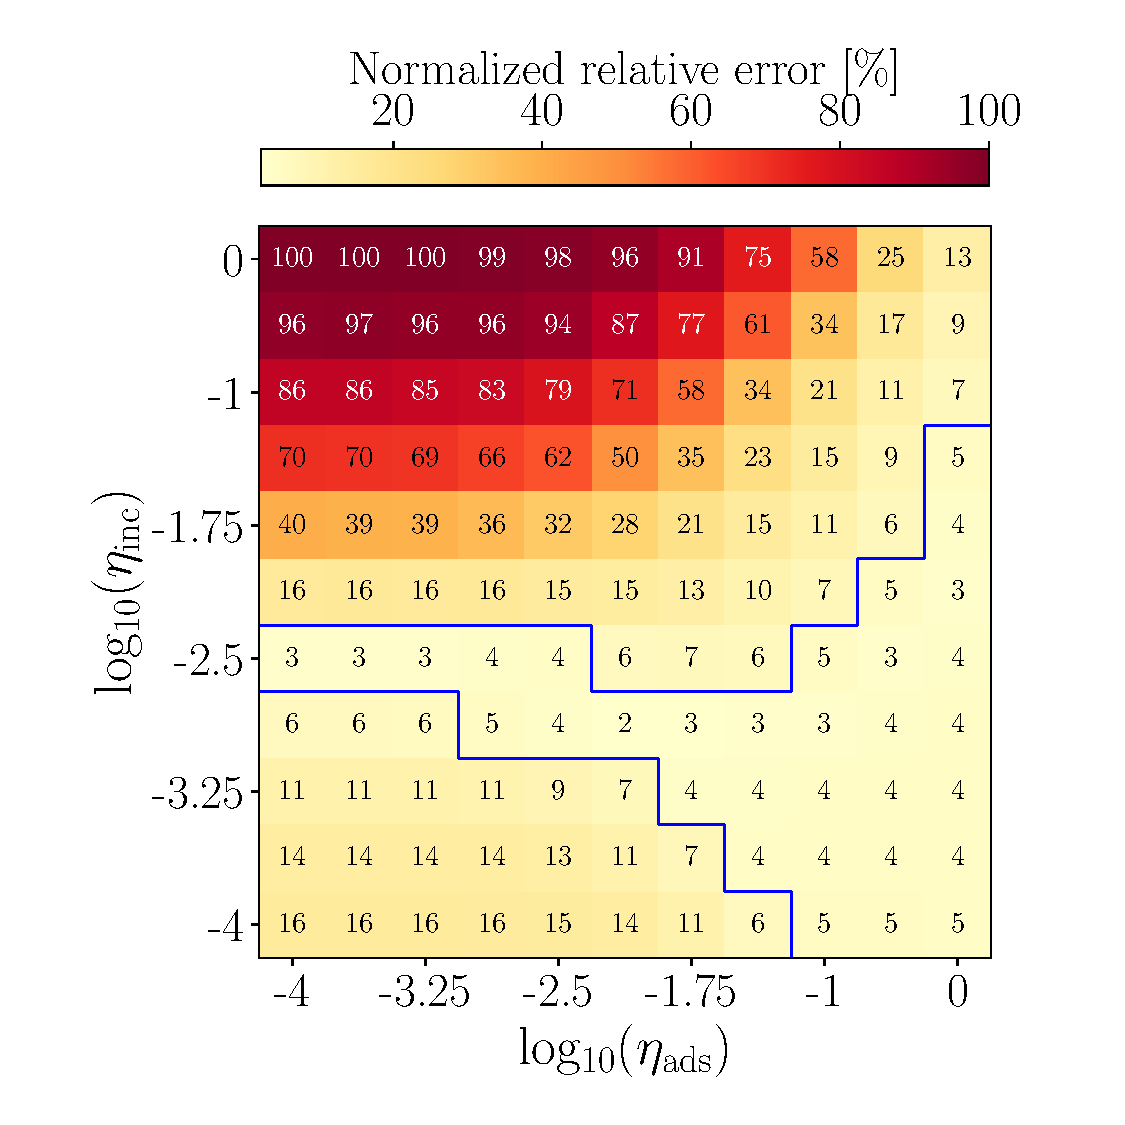
\includegraphics[width=0.5\textwidth]{Figures/Results/Shocktube/Agafonov2016_cpr/5CH4_norm_yield_error_readim.pdf}
	\caption{The relative error of carbon yield normalized by the maximum value at t=1.5 ms for 5\%~$\mathrm{CH_4}$ obtained using Caltech mechanism and Reactive Dimerization}.
	\label{fig:shockagof_yielderror_cpr} 
\end{figure}


%The model was run without soot (only the gas phase is simulated and no soot conversion allowed) to provide insight into the effect of temperature on the species involved in soot formation.

Figure~\ref{fig:SPC_cmf_cpr}-a shows the carbon mass fraction (CMF) of soot precursors (individual PAHs and total) and $\mathrm{C_2H_2}$ at 1.5 ms over the studied temperature range when soot model is deactivated. While the precursors exhibit a bell-shape behavior, the CMF of $\mathrm{C_2H_2}$ linearly increases with temperature and levels off after reaching 85\% $\mathrm{T_5\approx}$2400K. Among the considered PAHs, A2, A2R5, and A4R5 contain the majority of carbon and are expected to be major contributors to soot inception and surface growth.

\begin{figure}[H]
	\centering
	\begin{subfigure}[t]{0.4\textwidth}
		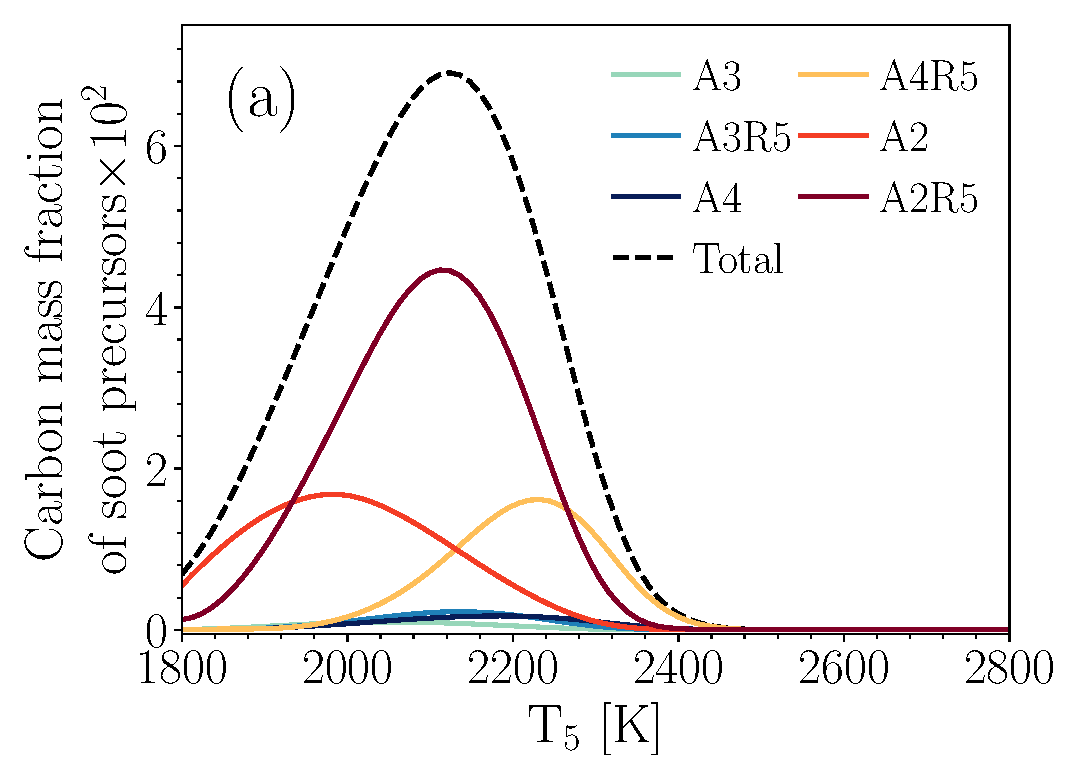
\includegraphics[width=1\textwidth]{Figures/Results/Shocktube/Agafonov2016_cpr/SPC_cmf_separate.pdf}
	\end{subfigure}
	\begin{subfigure}[t]{0.36\textwidth}
		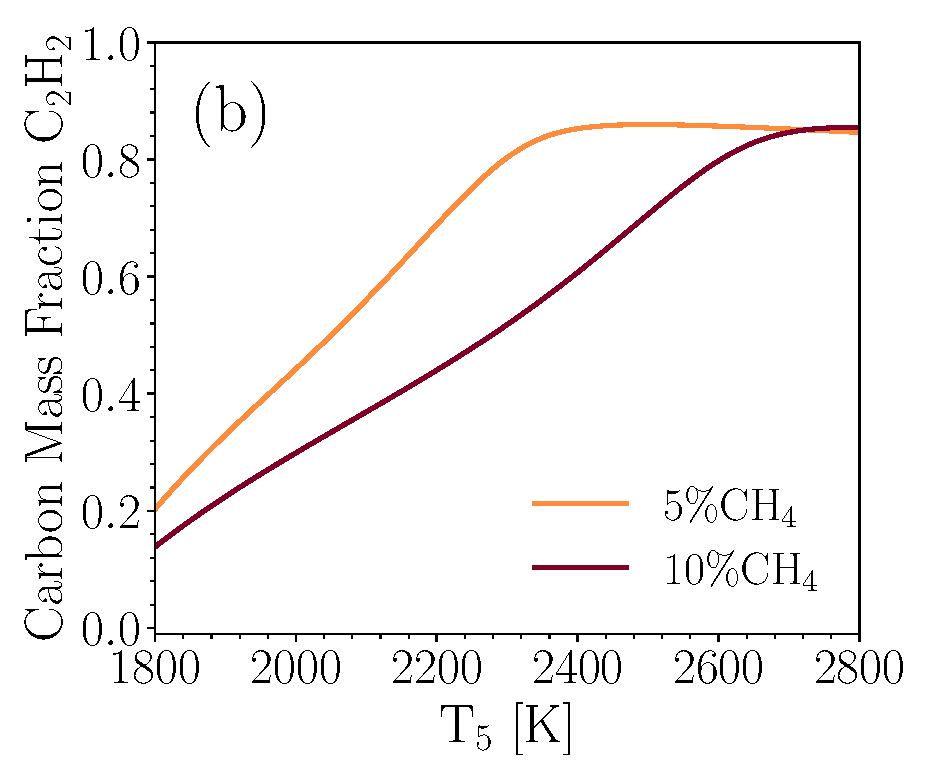
\includegraphics[width=1\textwidth]{Figures/Results/Shocktube/Agafonov2016_cpr/C2H2_cmf.pdf}
	\end{subfigure}
	\caption{The bell-shape temperature profile of carbon mass fraction of soot precursors (A2 and larger) combined (a) and $\mathrm{C_2H_2}$ (b) at t=1.5 ms during pyrolysis of 5\% (red line) and 10\%~$\mathrm{CH_4}$-Ar (green line) obtained using CPR model with Caltech mechanism without considering soot}
	\label{fig:SPC_cmf_cpr} 
\end{figure}

Next set of simulations were conducted by using equal adjustment factors ($\eta_{inc}=\eta_{ads}$) to minimize the prediction error of soot carbon yield. Figure~\ref{fig:shockagof_yield_dp_cpr} compares soot carbon yield and $d_p$ predicted using the different inception models and the sectional population balance model with the data from extinction measurements~\citep{agafonov2016unified}. A skew exponential curve (represented by the black dotted line) was fitted to the data to highlight the trend in carbon yield, and its likely peak at 12\%. Soot carbon yield has a bell-shape profile similar to the one shown for soot precursor because soot inception flux and mass growth are directly tied to the concentration of precursors used by the inception models. The yield predicted by Reactive Dimerization in the temperature range less than the temperature of the peak yield is larger than other inception models. EBridge Modified is shifted to higher temperatures compared to other inception models indicating different temperature dependence in this model, specifically the first step (PAH dehydrogenation) that is described by an Arrhenius rate as opposed to the other model where inception is initiated with physical collision of PAHs. The predicted $d_p$ uniformly increases with $\mathrm{T_5}$ to the peak value of 12.5 nm at 2700 K where yield is very low ($\approx10^{-7}$), and then rapidly falls to the minimum possible diameter in the model, 2 nm.

\begin{figure}[H]
	\centering
	\begin{tikzpicture}
		\draw (0, 0) node[inner sep=0] 	{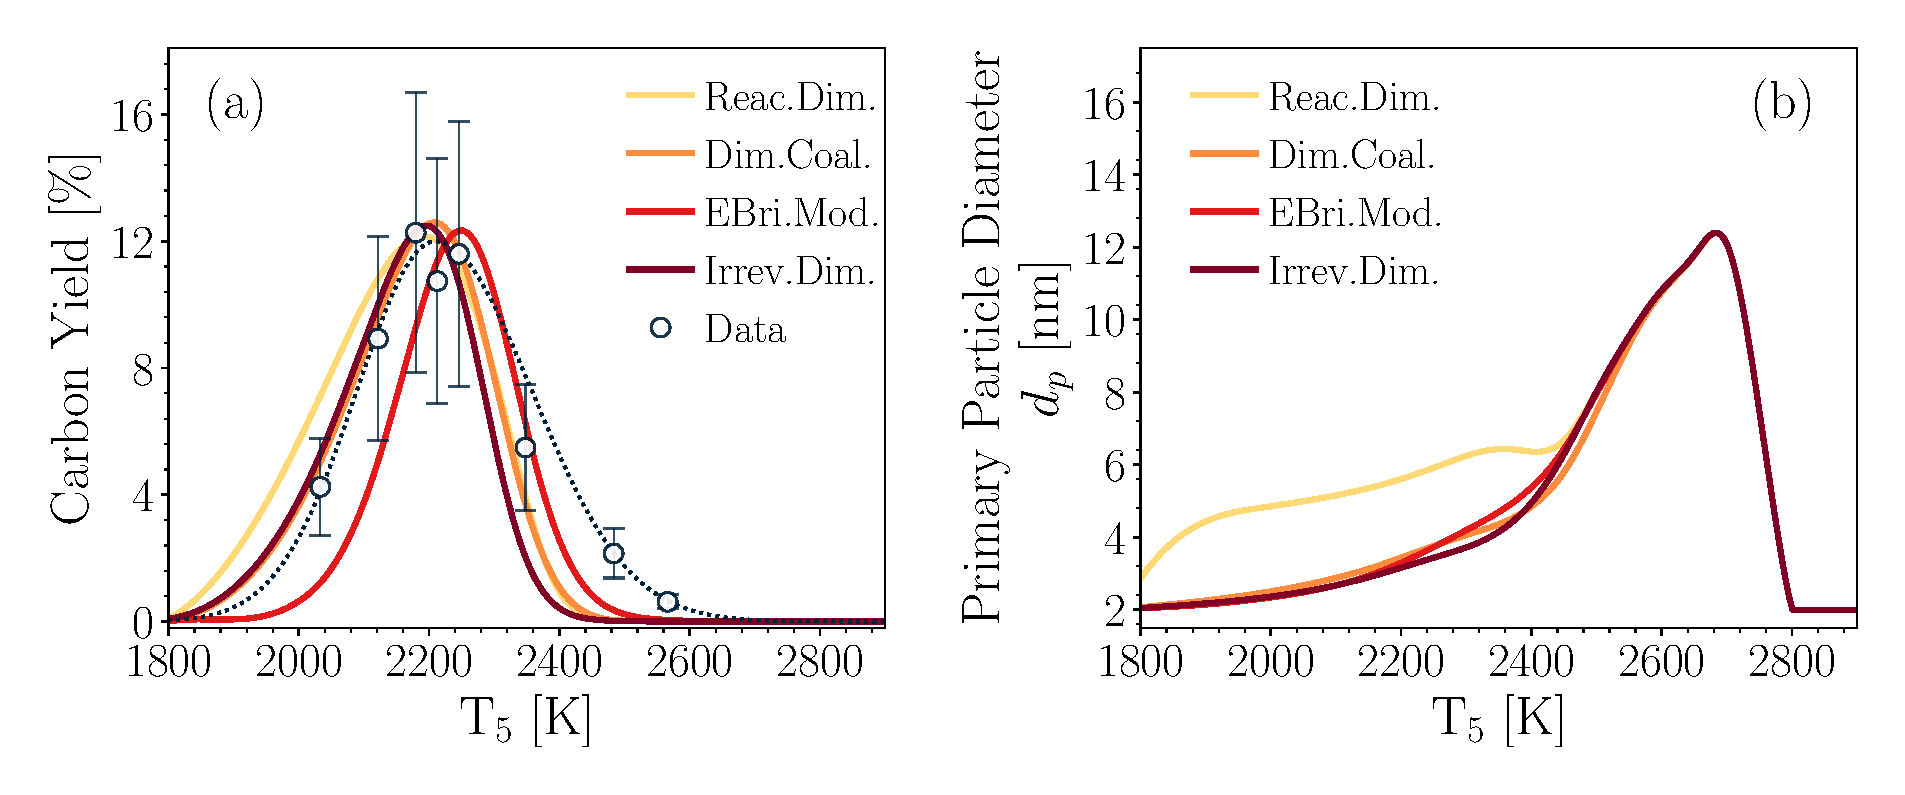
\includegraphics[width=0.8\textwidth]{Figures/Results/Shocktube/Agafonov2016_cpr/carbon_yield_d_p_5CH4.pdf}};
		\draw (-0.85, 0.42) node {\scriptsize{\cite{agafonov2016unified}}};
		%\draw (2.42, -0.23) node {\scriptsize{\cite{agafonov2016unified}}};
	\end{tikzpicture}
	\caption{The bell-shape temperature profile of soot carbon yield at t=1.5 ms (a) and increasing primary particle diameter, $d_p$ obtained using Caltech mechanism and different inception models optimized using equal adjustment factors to minimize the prediction with extinction measurements~\citep{agafonov2016unified}. The dashed line was added to show the trend in the measurements.}
	\label{fig:shockagof_yield_dp_cpr} 
\end{figure}


The differences of inception models in prediction of $d_p$  is overall negligible except for Reactive Dimerization, which predicts a larger $d_p$ in $\mathrm{T_5}<$2500. The $d_p$ trends can be better understood by examining Equation\eqref{eqn:d_p} indicating that $d_p$ is proportional of the third-root of $C_{tot}/N_{pri}$. $C_{tot}$ describes total carbon mass converted to soot through inception and surface growth while $N_{pri}$ is only determined by inception flux. As a result, $d_p$ is controlled by the ratio of surface growth (HACA and PAH adsorption) rate to inception flux. The ratio of carbon mass gained up to 1.5 ms by each pathway to the total soot carbon mass is calculated and shown in Figure\ref{fig:shockagof_carbon_map_cpr}. PAH adsorption is the dominant soot mass growth pathway for Reactive Dimerization in $\mathrm{T_5}<$2000 K (Figure\ref{fig:shockagof_carbon_map_cpr}-a) that results in larger $C_{tot}/N_{pri}$ and $d_p$ values, but inception is dominant for the other inception models. The carbon mass fraction of inception decreases with temperature for all inception models leading to higher $d_p$ values up to 2700 K and it increases afterwards that changes $d_p$ trends.


\begin{figure}[H]
	\centering
	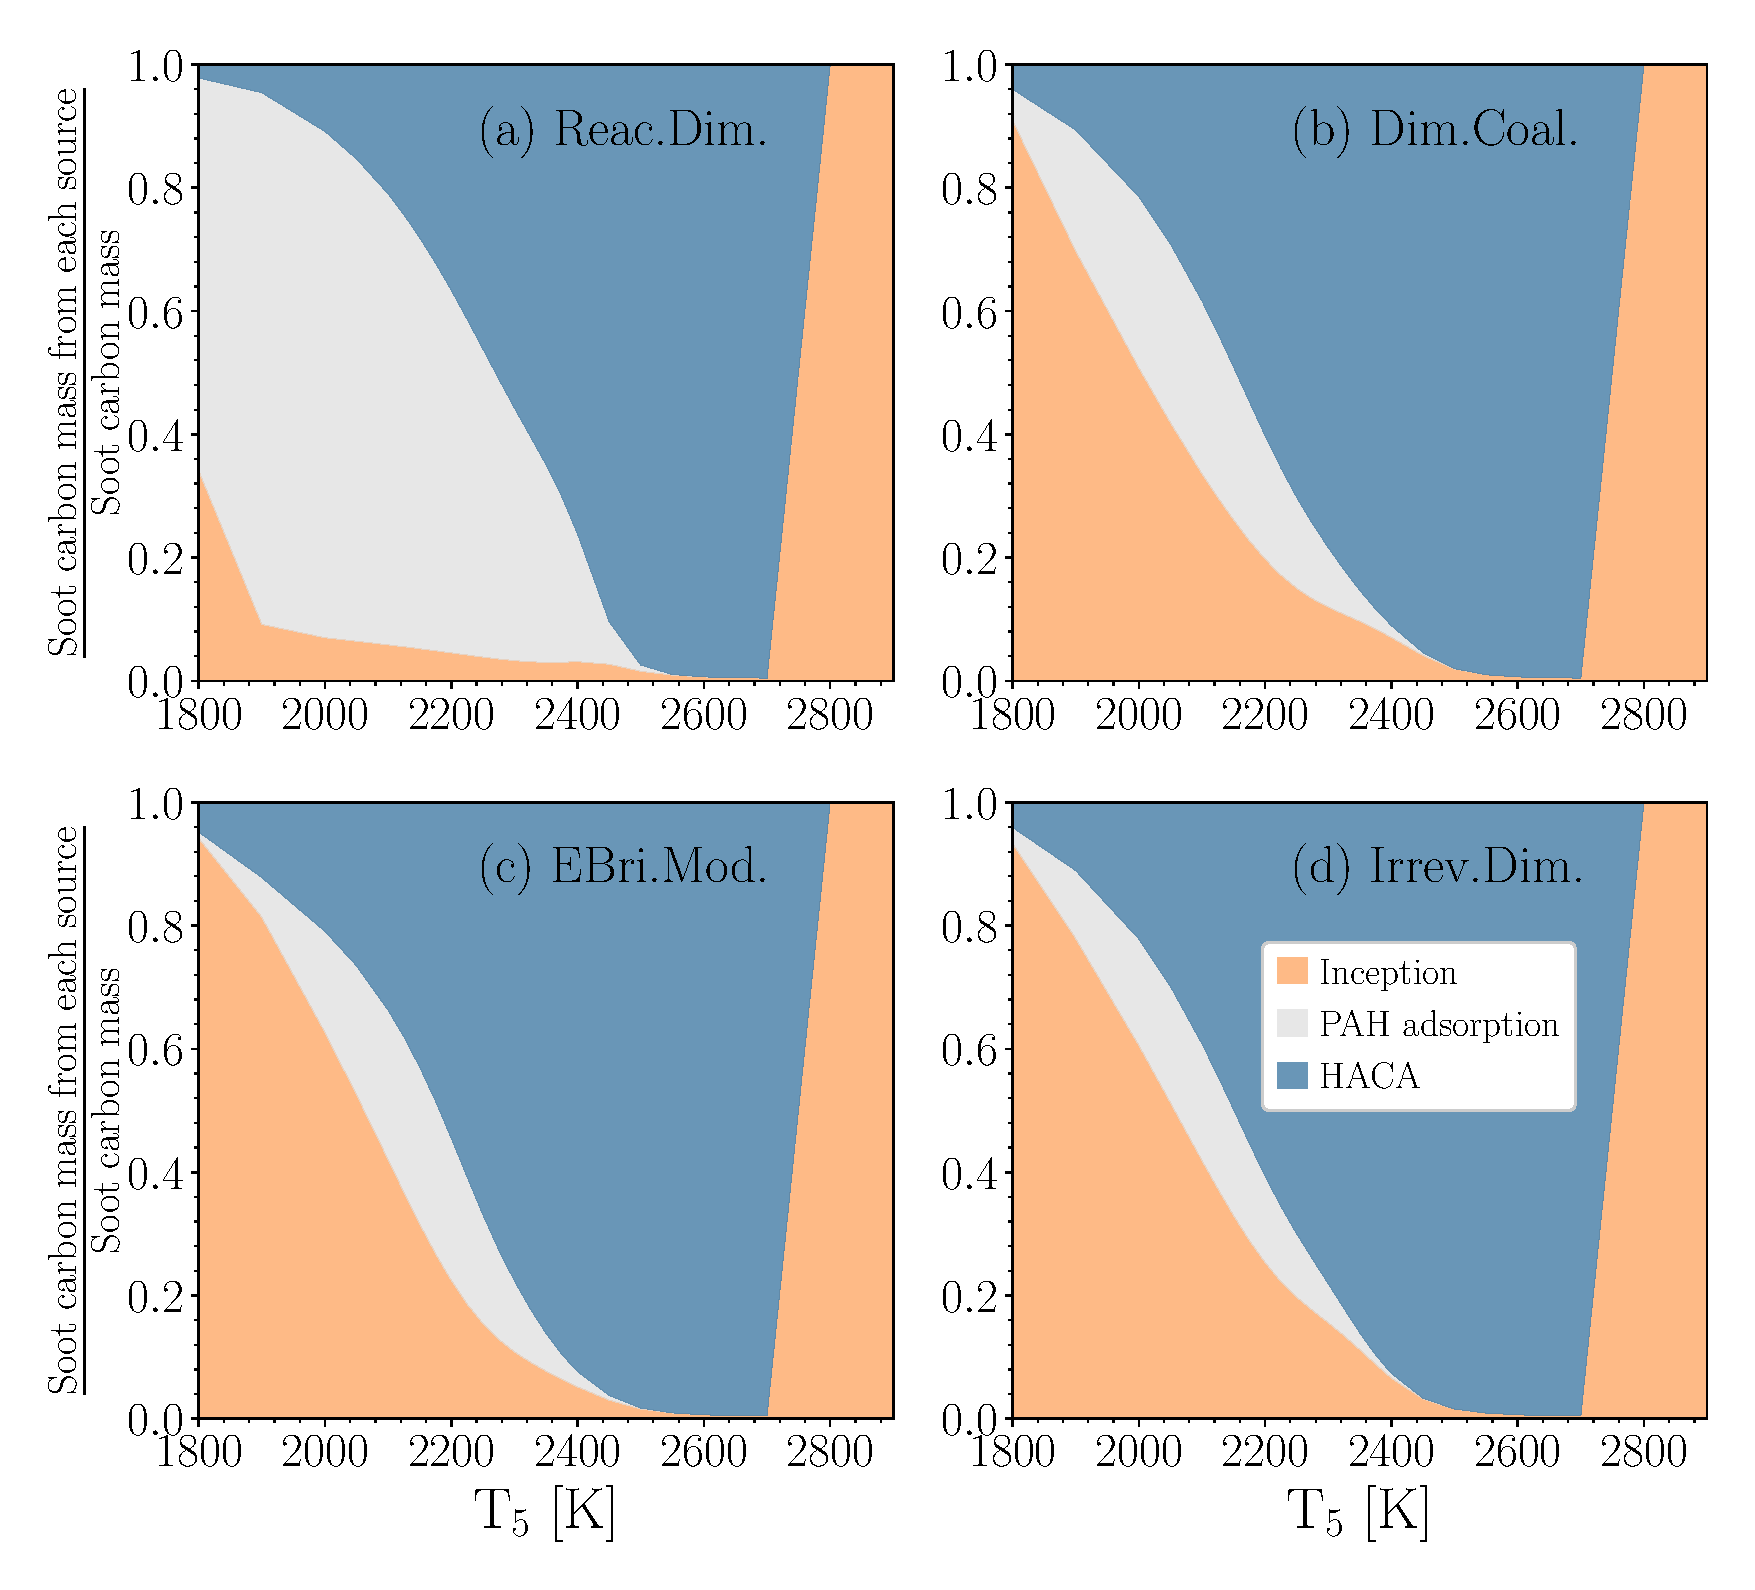
\includegraphics[width=0.8\textwidth]{Figures/Results/Shocktube/Agafonov2016_cpr/C_tot_distmap_5CH4.pdf}
	\caption{The soot carbon mass from inception, PAH adsorption and HACA normalized by total soot carbon mass at t=1.5 ms for 5\% in Ar obtained using Caltech mechanism and different inception models calibrated to minimize the prediction with extinction measurements~\citep{agafonov2016unified}.}
	\label{fig:shockagof_carbon_map_cpr} 
\end{figure}

As shown in Figure\ref{fig:shockagof_yield_maxincads_cpr}, the inception models optimized using the minimum inception ($\eta_{inc}$) and PAH adsorption ($\eta_{ads}$) adjustment factors result in the carbon yield values indistinguishably close except for EBridge Modified model that is slightly shifted to higher temperatures in both cases. The minimum adsorption case has a higher peak and a narrower profile compared the minimum inception. Figure\ref{fig:shockagof_yield_maxincads_cpr} demonstrates the variation in $d_p$ among the inception models with the minimum inception (solid line) mode compared to the minimum adsorption (dashed line) that show negligible sensitivity to the inception model. In the minimum inception mode, the majority of soot mass comes from PAHs, so $d_p$ shows a bell-shape profile with a peak close to the temperature of CMF of precursors (dashed line in Figure\ref{fig:SPC_cmf_cpr}). Reactive Dimerization has the largest variation at the peak from 2 to 21 nm for the minimum inception and adsorption, respectively. The global adjustment factors were used to alter the contribution of precursors to inception and surface growth without changing the internal rate constants of inception models. A close agreement was achieved between the predicted and measured carbon yield in different modes of inception and PAH adsorption that can result in different soot morphology. Characterizing primary particle size in the experiment can reduce the uncertainty in the model and restrict the range of expected inception and surface growth rate and highlight the need to account for missing pathways and phenomena involved in soot yield and morphology.

\begin{figure}[H]
	\centering
	\begin{tikzpicture}
			\draw (0, 0) node[inner sep=0] 	{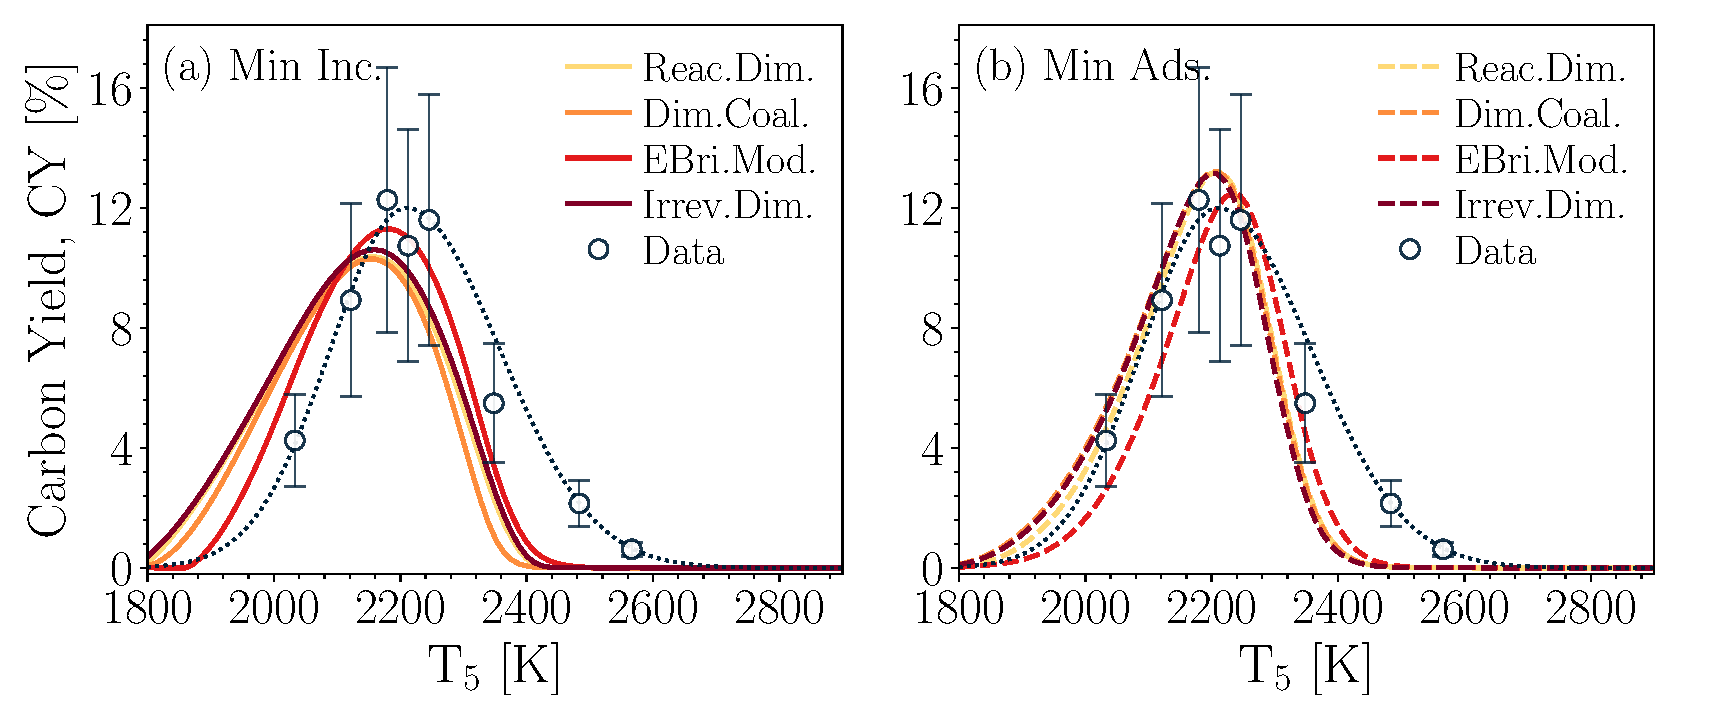
\includegraphics[width=0.8\textwidth]{Figures/Results/Shocktube/Agafonov2016_cpr/carbon_yield_maxincads_combined.pdf}};
			\draw (-0.48, 0.75) node {\scriptsize{\cite{agafonov2016unified}}};
			\draw (5.33, 0.75) node {\scriptsize{\cite{agafonov2016unified}}};
		\end{tikzpicture}
	\caption{The comparison of soot carbon yield at t=1.5 ms when the minimum inception (a) and the minimum PAH adsorption (b) adjustment factors were applied to minimized the prediction error compared to measurements~\citep{agafonov2016unified} for 5\%~$\mathrm{CH_4}$-Ar obtained using Caltech mechanism and different inception models.}
	\label{fig:shockagof_yield_maxincads_cpr} 
\end{figure}

%\begin{figure}[H]
%	\centering
%	\begin{tikzpicture}
%		\draw (0, 0) node[inner sep=0] 	{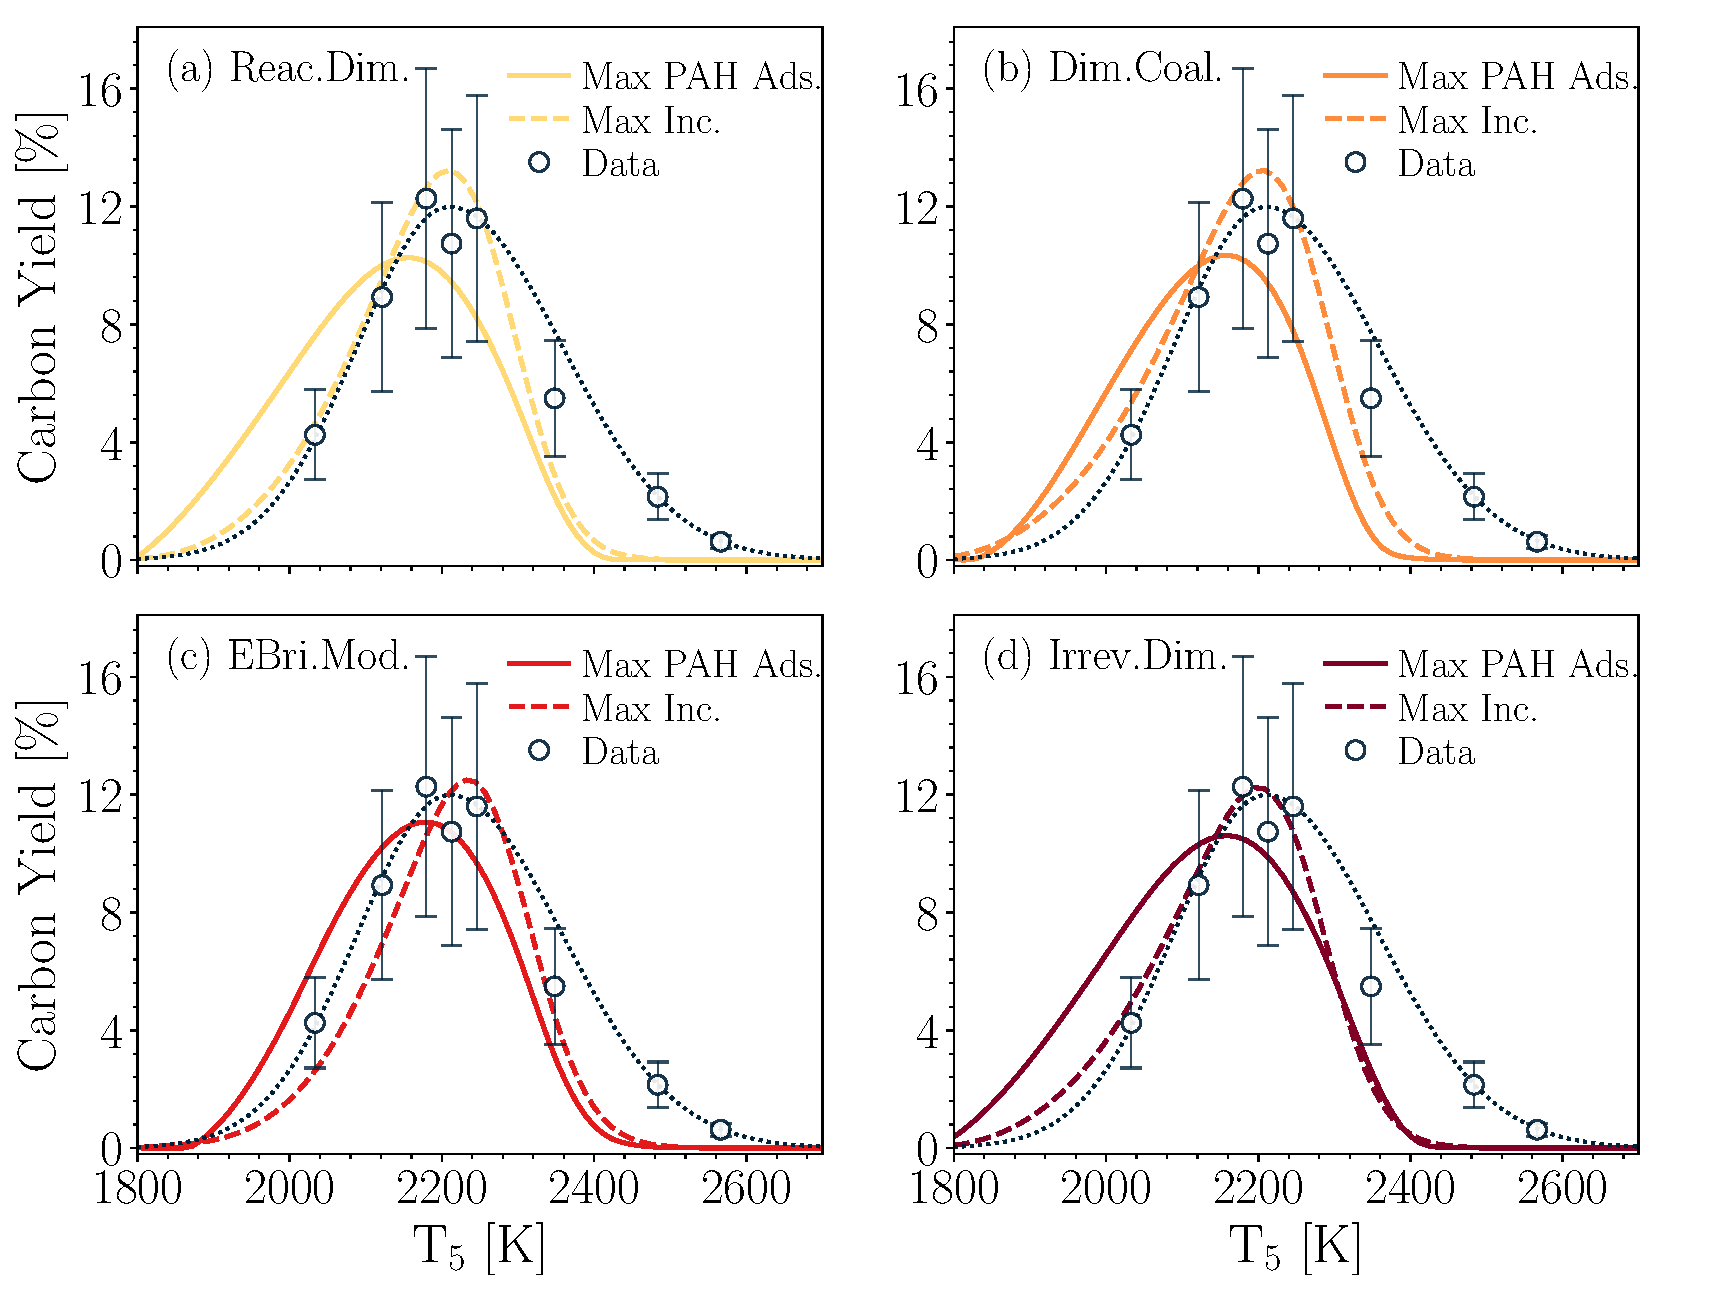
\includegraphics[width=0.8\textwidth]{Figures/Results/Shocktube/Agafonov2016_cpr/carbon_yield_maxincads.pdf}};
%		\draw (-0.48, -0.8) node {\scriptsize{\cite{agafonov2016unified}}};
%		\draw (5.33, -0.8) node {\scriptsize{\cite{agafonov2016unified}}};
%		\draw (-0.48, 3.36) node {\scriptsize{\cite{agafonov2016unified}}};
%		\draw (5.33, 3.36) node {\scriptsize{\cite{agafonov2016unified}}};
%	\end{tikzpicture}
%	\caption{The comparison of soot carbon yield at t=1.5 ms when maximum inception (dashed line) and PAH adsorption (solid line) were applied to minimized the prediction error compared to measurements~\citep{agafonov2016unified} for 5\% (a) and 10\%~$\mathrm{CH_4}$ (b) in Ar obtained using Caltech mechanism and different inception models.}
%	\label{fig:shockagof_yield_maxincads_cpr} 
%\end{figure}

\begin{figure}[H]
	\centering
	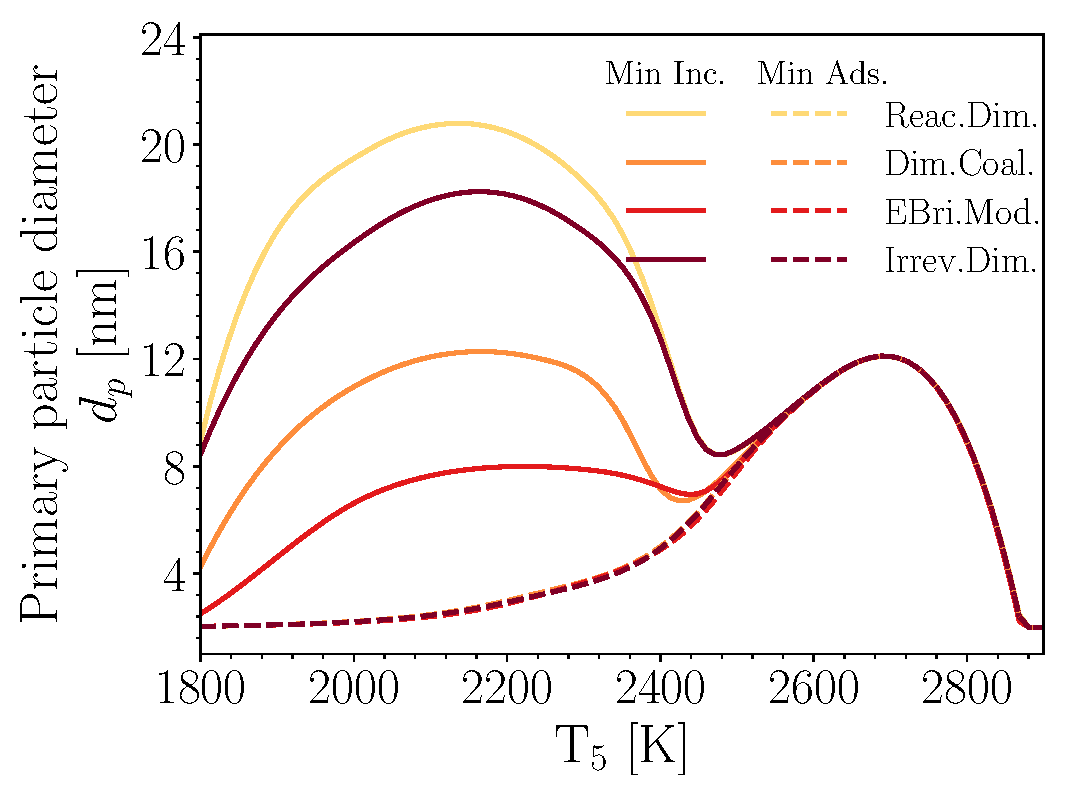
\includegraphics[width=0.5\textwidth]{Figures/Results/Shocktube/Agafonov2016_cpr/d_p_maxincads_combined.pdf}
	\caption{The comparison of mean primary particle, $d_p$ at t=1.5 ms when the minimum inception (solid lines) and adsorption (dashed lines) were applied to minimized the prediction error compared to measurements~\citep{agafonov2016unified} for 5\%-Ar obtained using Caltech mechanism and different inception models.}
	\label{fig:shockagof_dp_maxincads_cpr} 
\end{figure}

%\begin{figure}[H]
%	\centering
%	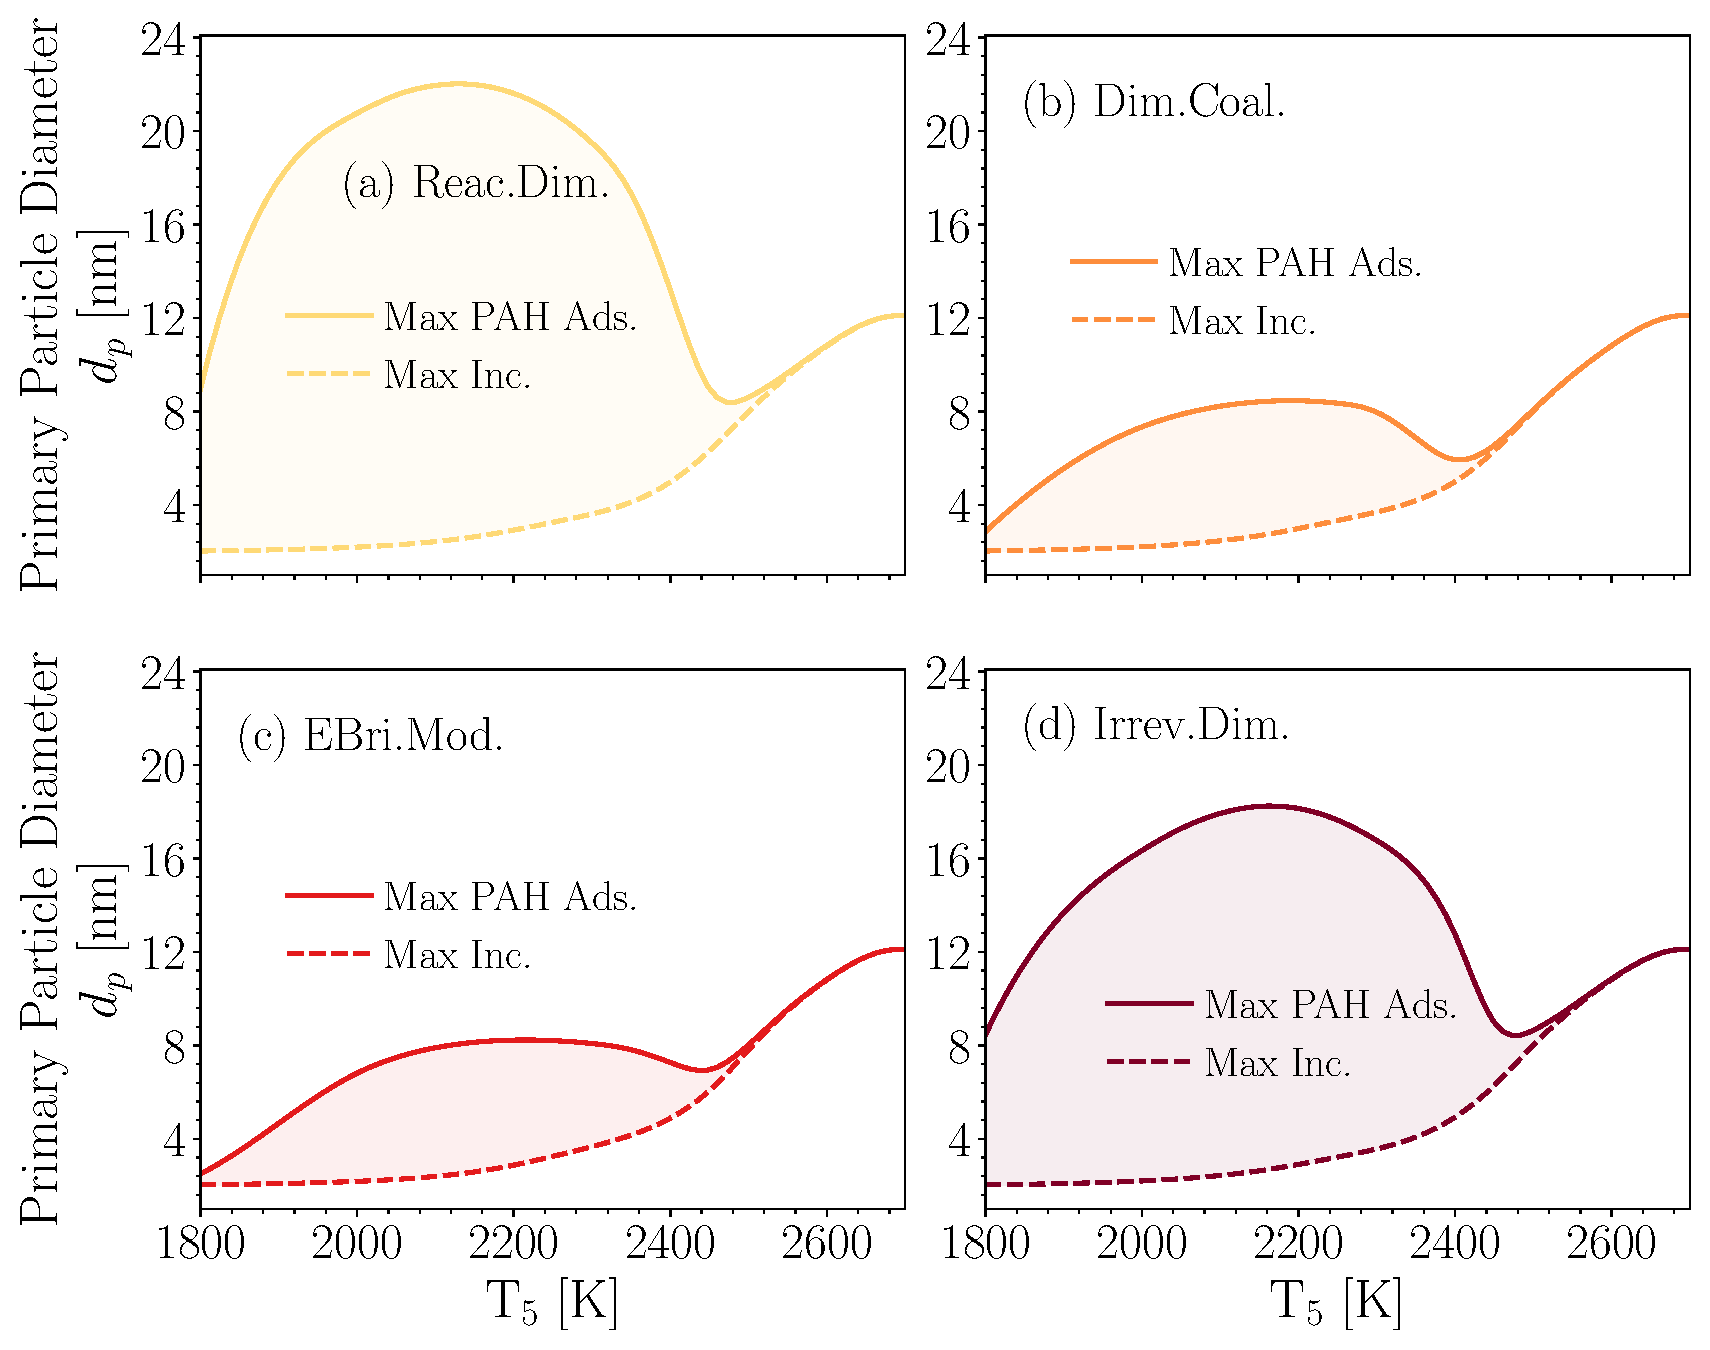
\includegraphics[width=0.8\textwidth]{Figures/Results/Shocktube/Agafonov2016_cpr/d_p_maxincads.pdf}
%	\caption{The comparison of mean primary particle, $d_p$ at t=1.5 ms when maximum inception and PAH adsorption were applied to minimized the prediction  error compared to measurements~\citep{agafonov2016unified} for 5\% (a) and 10\%~$\mathrm{CH_4}$ (b) in Ar obtained using Caltech mechanism and different inception models.}
%	\label{fig:shockagof_dp_maxincads_cpr} 
%\end{figure}

%\subsection{Methane pyrolysis in shock-tube using constant volume reactor}

%The pyrolysis of 5\% and 10\% $\mathrm{CH_4}$-Ar was investigated using a constant volume reactor model (CVR) for the post-shock temperature, $T_5$ range of 1800-3000 K, and pressure, $P_5$ range of 4.7-7.1 bar. $P_5$ was assumed to linearly increase with $T_5$ across the simulation cases. Caltech mechanism was used and the inception models were calibrated in order to match carbon yield at t=1.5 ms with the measurement~\citep{agafonov2016unified} using a dual-beam absorption–emission technique. \citet{agafonov2016unified} reported yield$\times$E(m) at $\mathrm{\lambda}$=632~nm, and yield data was retrieved using E(m)=0.37 suggested therein. 


%\begin{figure}[H]
%	\centering
%	\begin{subfigure}[t]{0.4\textwidth}
%		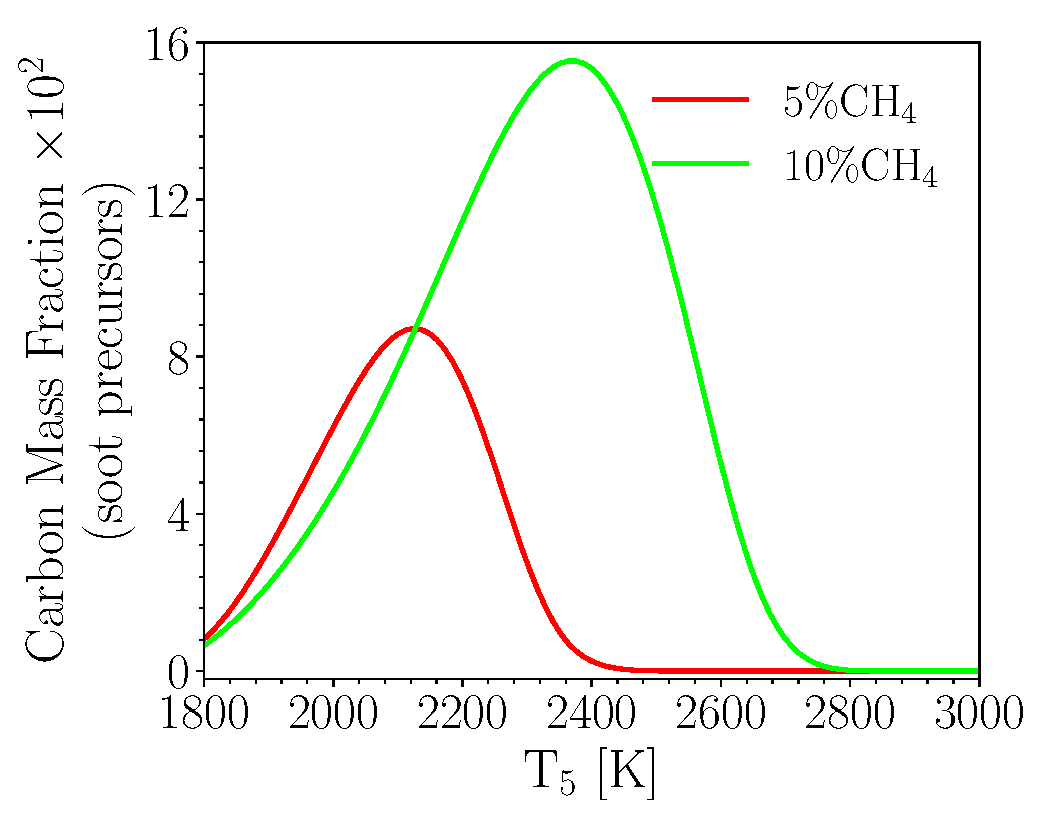
\includegraphics[width=1\textwidth]{Figures/Results/Shocktube/Agafonov2016_cvr/SPC_cmf.pdf}
%	\end{subfigure}
%	\begin{subfigure}[t]{0.4\textwidth}
%		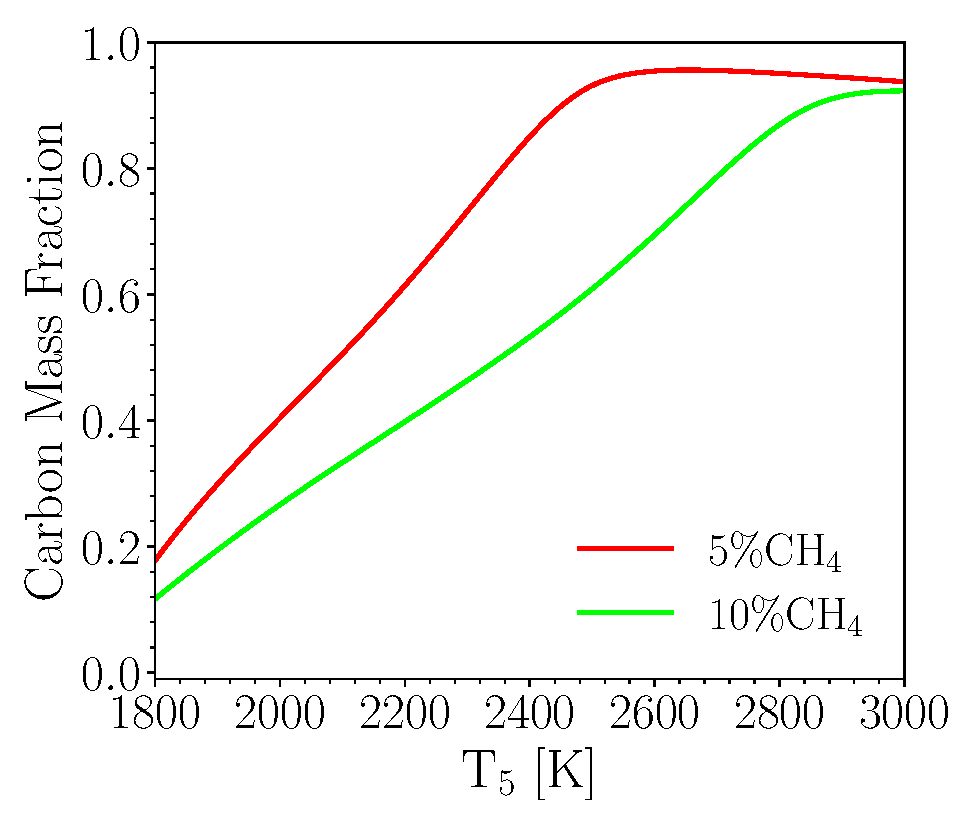
\includegraphics[width=1\textwidth]{Figures/Results/Shocktube/Agafonov2016_cvr/C2H2_cmf.pdf}
%	\end{subfigure}
%	\caption{The bell-shape temperature profile of carbon mass fraction of soot precursors (A2 and larger) combined (a) and $\mathrm{C_2H_2}$ (b) at t=1.5 ms during pyrolysis of 5\% (red line) and 10\%~$\mathrm{CH_4}$-Ar (green line) obtained using Caltech mechanism without considering soot}
%	\label{fig:SPC_cmf_cvr} 
%\end{figure}
%
%
%
%
%\begin{figure}[H]
%	\centering
%	\begin{tikzpicture}
%		\draw (0, 0) node[inner sep=0] 	{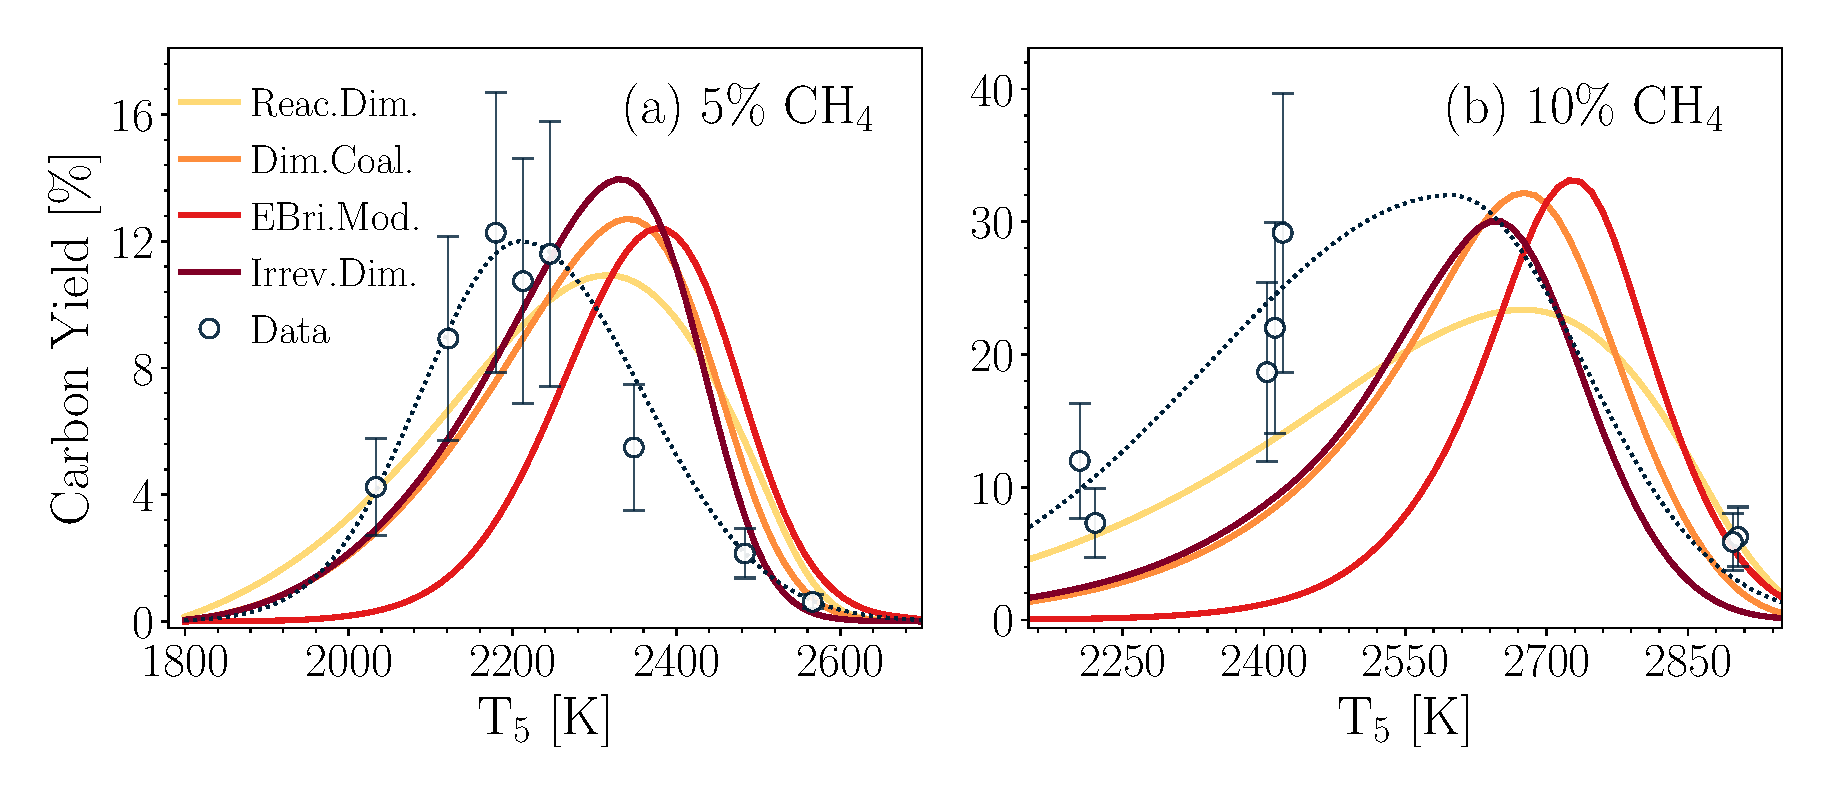
\includegraphics[width=0.8\textwidth]{Figures/Results/Shocktube/Agafonov2016_cvr/carbon_yield.pdf}};
%		\draw (-3.6, 0.42) node {\scriptsize{\cite{agafonov2016unified}}};
%		%\draw (2.42, -0.23) node {\scriptsize{\cite{agafonov2016unified}}};
%	\end{tikzpicture}
%	\caption{The bell-shape temperature profile of soot carbon yield at t=1.5 ms for 5\% (a) and 10\%~$\mathrm{CH_4}$ (b) in Ar obtained using Caltech mechanism and different inception models calibrated to minimize the prediction with extinction measurements~\citep{agafonov2016unified}.}
%	\label{fig:shockagof_yield_cvr} 
%\end{figure}
%
%Figure~\ref{fig:shockagof_yield} shows soot carbon yield predicted using Caltech mechanism where inception flux and PAH adsorption rate were adjusted using a scaling factor (equal for the both) to minimize the prediction error compared to the data from extinction measurements~\citep{agafonov2016unified}. A skew exponential curve fit (represented by the black dotted line) was applied to illustrate the trend in soot yield and identify the temperature at which the yield likely reaches its maximum. The predicted temperature of peak yield is larger than peak of curve-fit in both $\mathrm{CH_4}$ concentrations by 100-200 K depending on the inception model. This difference is due the contribution of  HACA to surface growth that depends on $\mathrm{C_2H_2}$ concentration which increases with temperature.
%
%\begin{figure}[H]
%	\centering
%	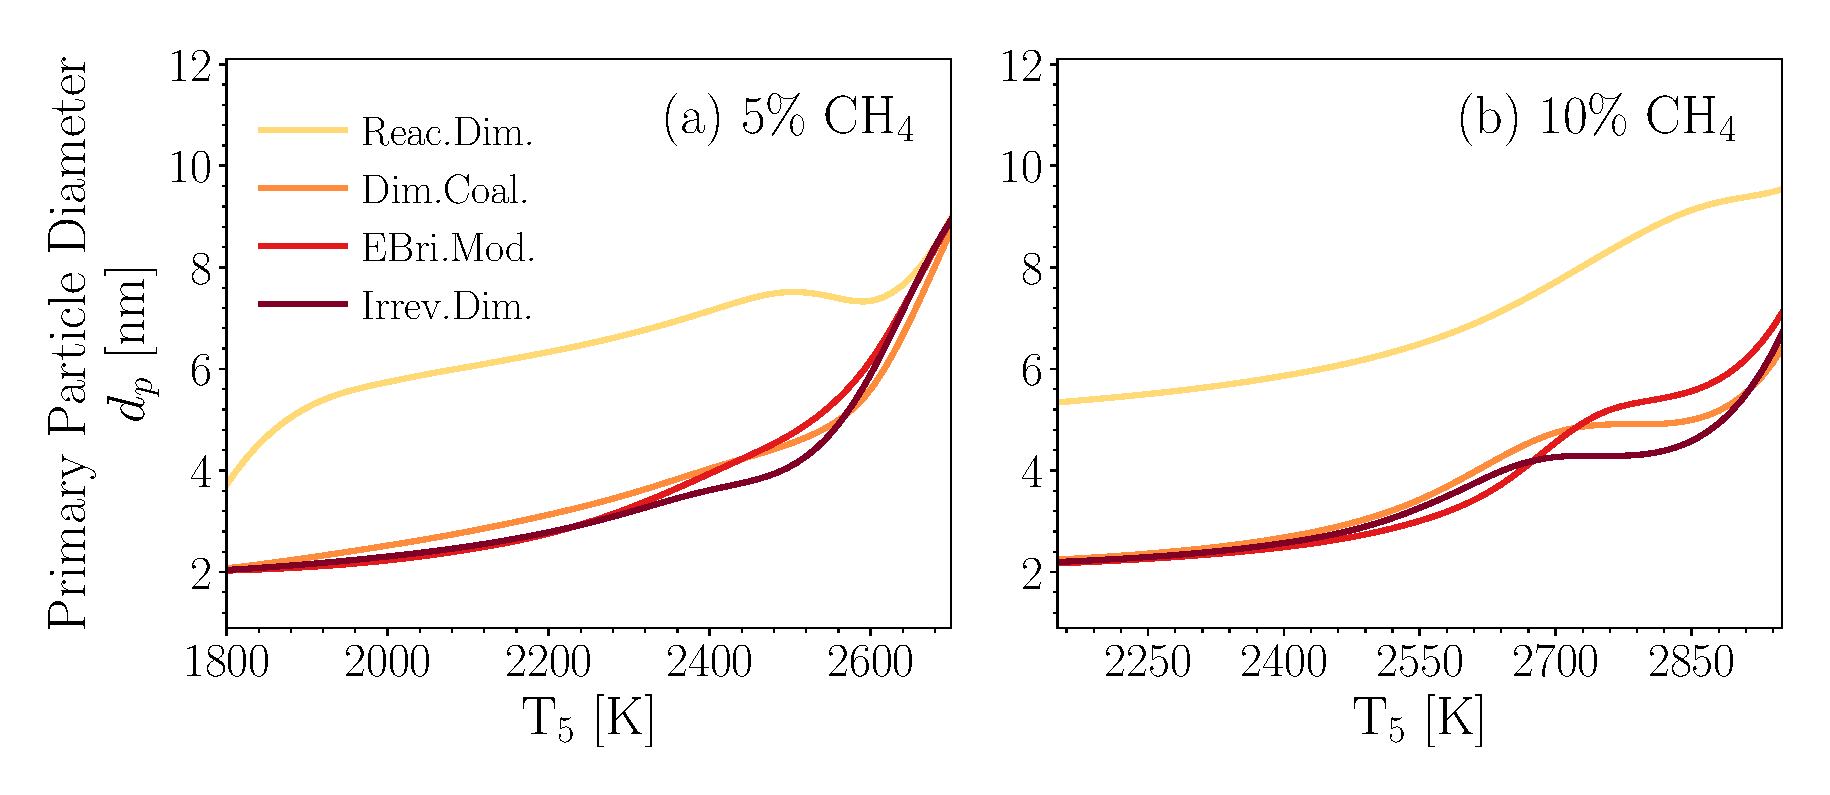
\includegraphics[width=0.8\textwidth]{Figures/Results/Shocktube/Agafonov2016_cvr/d_p.pdf}
%	\caption{The temperature dependence of mean primary particle diameter, $d_p$ at t=1.5 ms for 5\% (a) and 10\%~$\mathrm{CH_4}$ (b) in Ar obtained using Caltech mechanism and different inception models calibrated to minimize the prediction with extinction measurements~\citep{agafonov2016unified}.}
%	\label{fig:shockagof_dp_cvr} 
%\end{figure}
%
%Figure\ref{fig:shockagof_dp} shows that $d_p$ increases with temperature up to 10 nm. For 5\% $\mathrm{CH_4}$, $d_p$ reaches the peak around 2800 K and drops quickly to 2 nm which is the minimum allowed diameter in the model. Reactive Dimerization results in overall larger primary particle diameters, but the behavior of the rest of inception models are similar.
%
%\begin{figure}[H]
%	\centering
%	\begin{tikzpicture}
%		\draw (0, 0) node[inner sep=0] 	{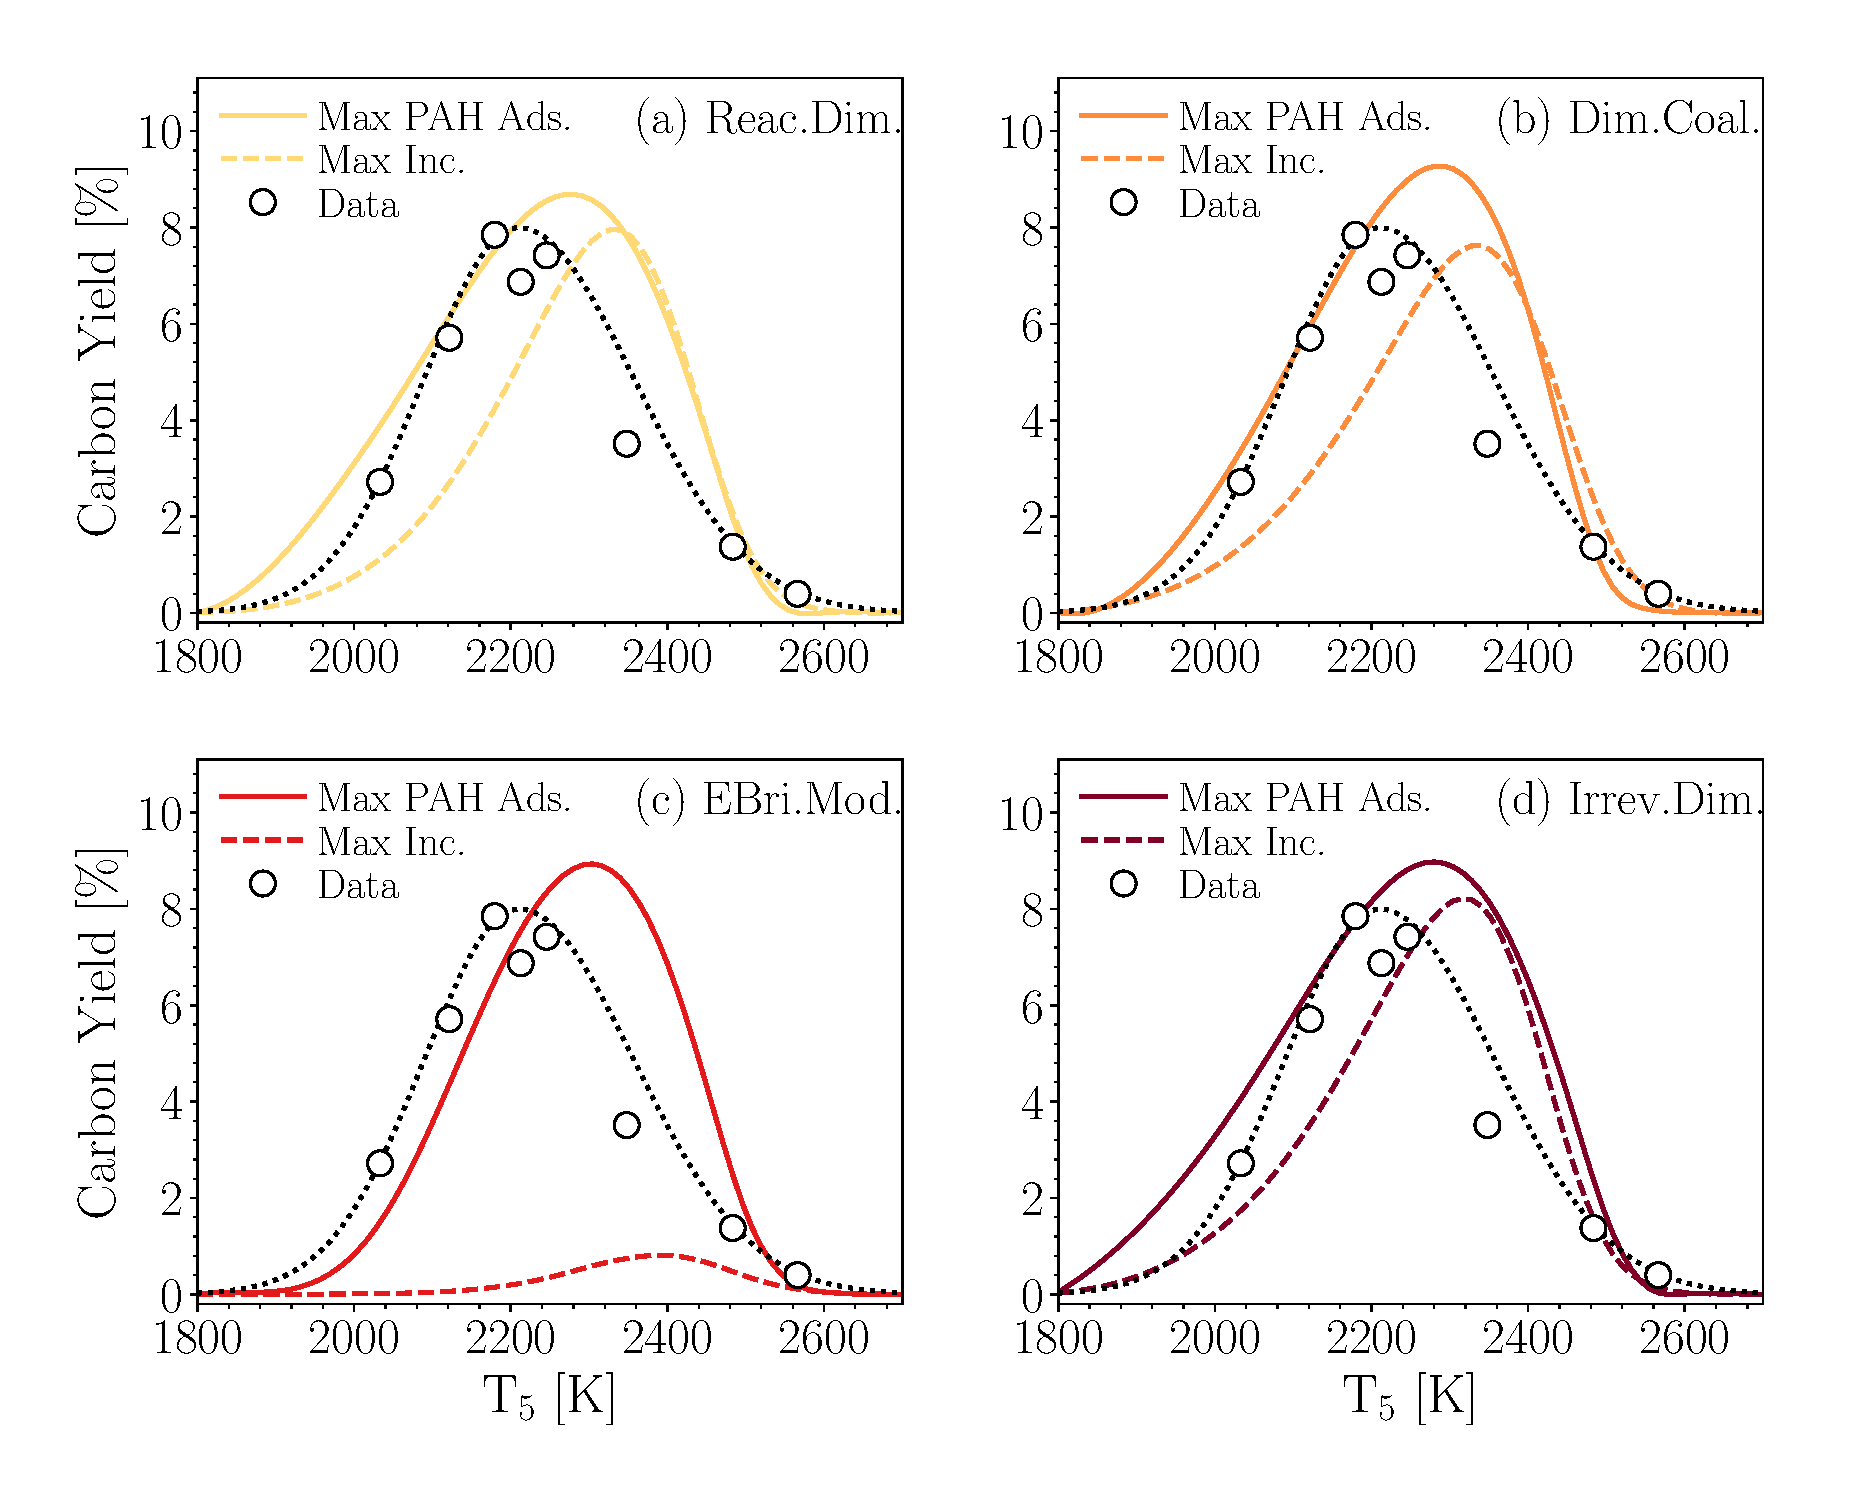
\includegraphics[width=0.8\textwidth]{Figures/Results/Shocktube/Agafonov2016_cvr/carbon_yield_maxincads.pdf}};
%		\draw (-3.18, -0.9) node {\scriptsize{\cite{agafonov2016unified}}};
%		\draw (2.46, -0.9) node {\scriptsize{\cite{agafonov2016unified}}};
%		\draw (-3.18, 3.55) node {\scriptsize{\cite{agafonov2016unified}}};
%		\draw (2.46, 3.55) node {\scriptsize{\cite{agafonov2016unified}}};
%	\end{tikzpicture}
%	\caption{The comparison of soot carbon yield at t=1.5 ms when maximum inception and PAH adsorption were applied to minimized the prediction  error compared to measurements~\citep{agafonov2016unified} for 5\% (a) and 10\%~$\mathrm{CH_4}$ (b) in Ar obtained using Caltech mechanism and different inception models.}
%	\label{fig:shockagof_yield_maxincads_cvr} 
%\end{figure}
%
%\begin{figure}[H]
%	\centering
%	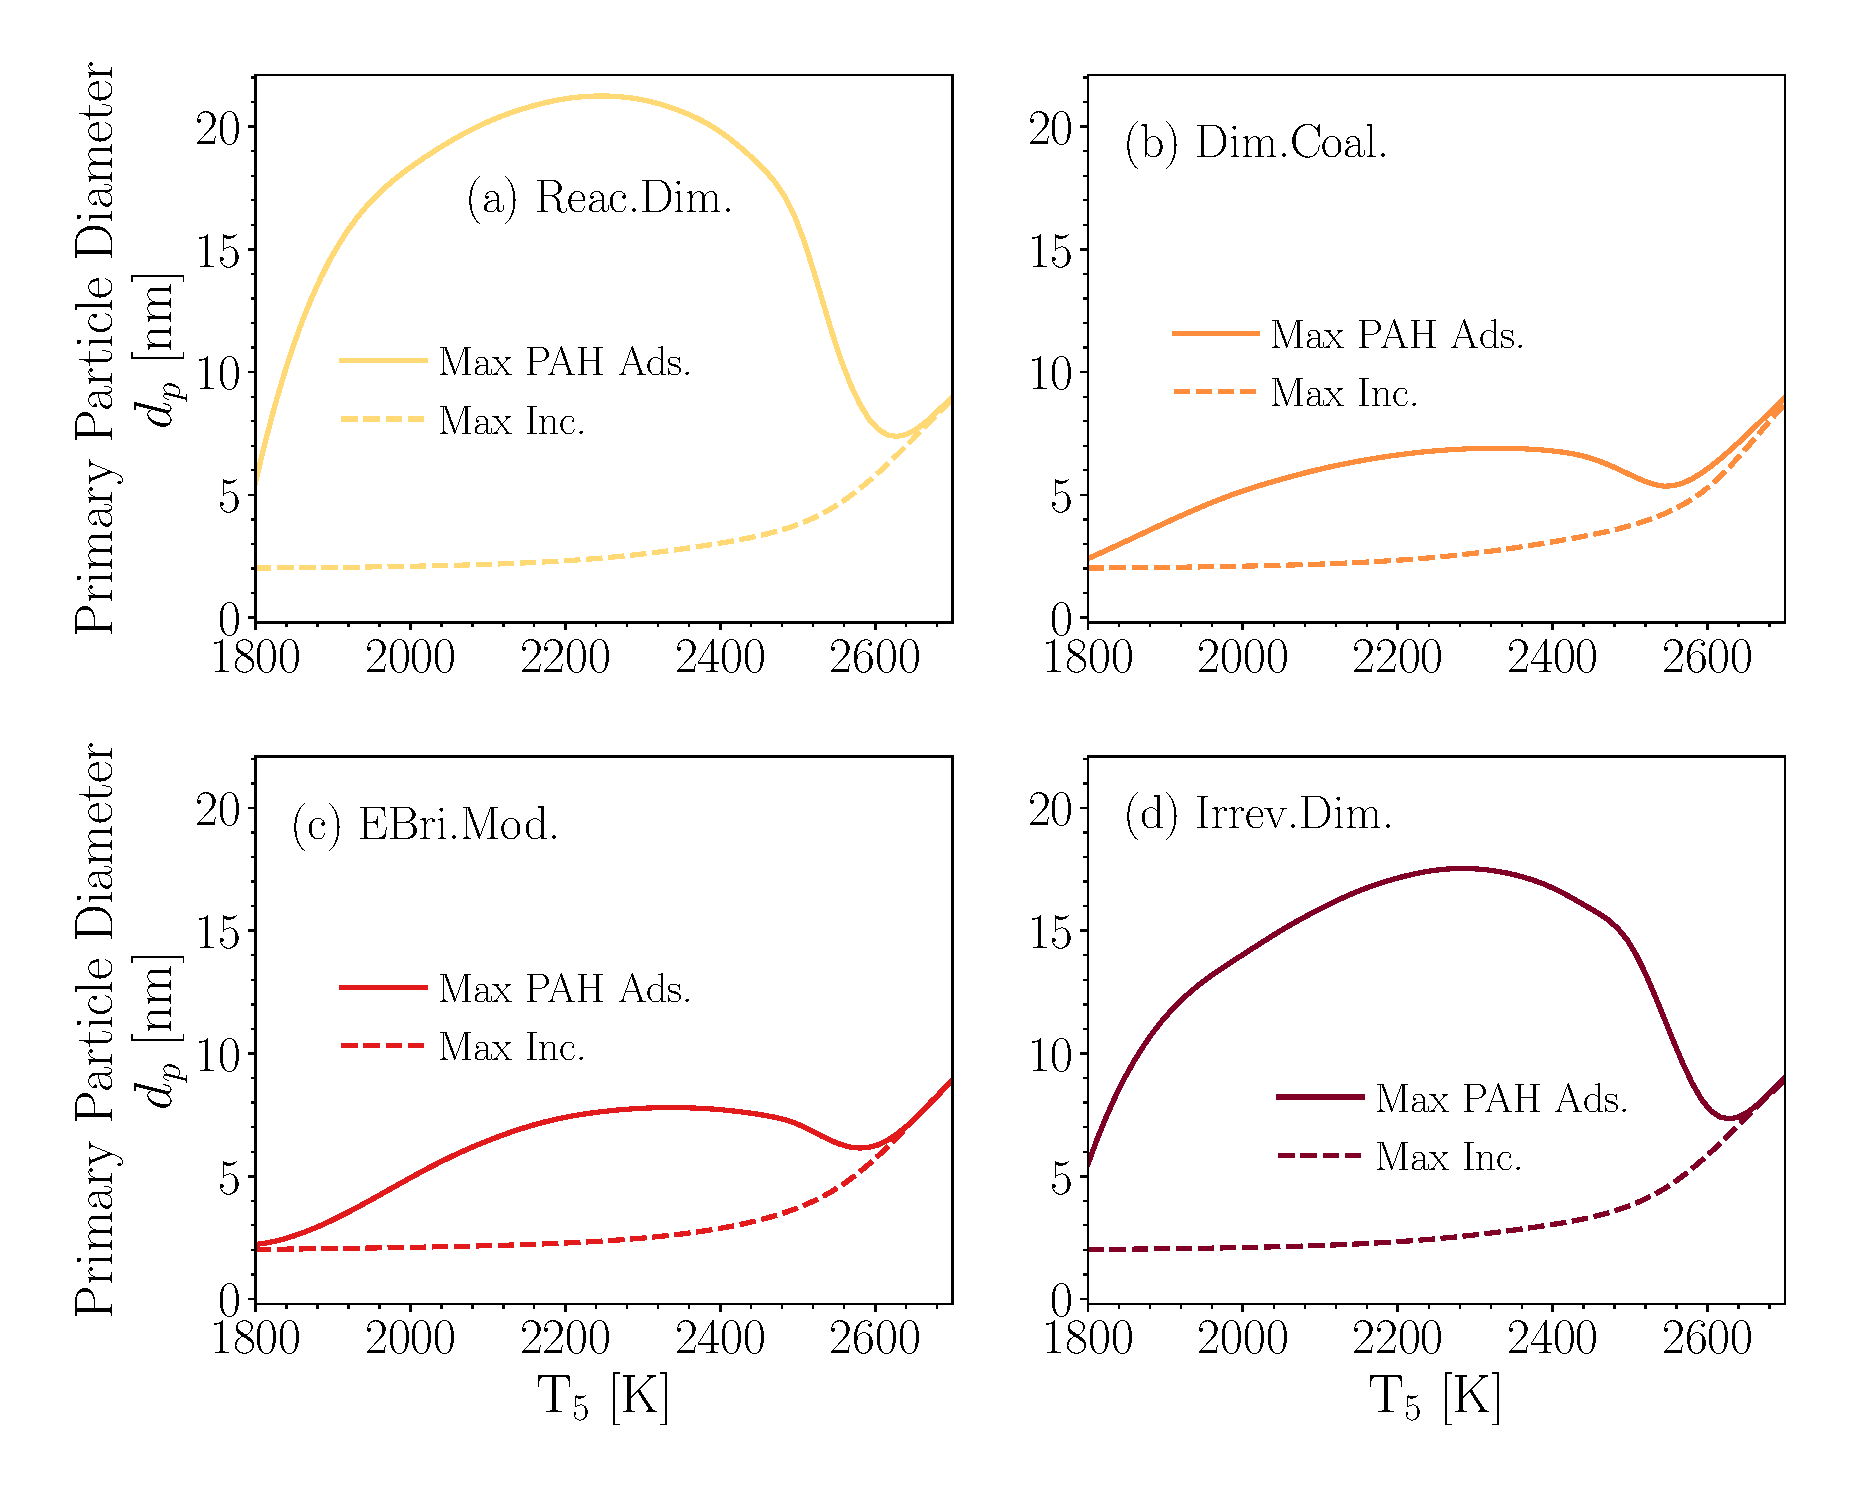
\includegraphics[width=0.8\textwidth]{Figures/Results/Shocktube/Agafonov2016_cvr/d_p_maxincads.pdf}
%	\caption{The comparison of mean primary particle, $d_p$ at t=1.5 ms when maximum inception and PAH adsorption were applied to minimized the prediction  error compared to measurements~\citep{agafonov2016unified} for 5\% (a) and 10\%~$\mathrm{CH_4}$ (b) in Ar obtained using Caltech mechanism and different inception models.}
%	\label{fig:shockagof_dp_maxincads_cvr} 
%\end{figure}